{ %section2_1
	\subsection{Параллельное ускорение и параллельная эффективность}
	\parДля оценки эффективности параллельной программы принято сравнивать показатели скорости исполнения этой программы при её запуске на нескольких идентичных вычислительных системах, которые различаются только количеством центральных процессоров (или ядер). На практике, однако, редко используют для этой цели несколько независимых аппаратных платформ, т.к. обеспечить их полную идентичность по всем параметрам достаточно сложно. Вместо этого, измерения проводятся на одной многопроцессорной (многоядерной) вычислительной системе, в которой искусственно ограничивается количество процессоров (ядер), задействованных в вычислениях. Это обычно достигается одним из следующих способов:
	\begin{itemize}
		\itemУстановка аффинности процессоров (ядер).
		\itemВиртуализация процессоров (ядер).
		\itemУправление количеством нитей.
	\end{itemize}
	\textbf{Установка аффинности.} Под аффинностью (processor affinity/pinning) понимается указание операционной системе запускать указанный поток/про-\\цесс на явно заданном процессоре (ядре). Установить аффинность можно либо с помощью специального системного вызова изнутри самой параллельной программы, либо некоторым образом извне параллельной программы (например, средствами ''Диспетчера задач'' или с помощью команды ''start'' с ключом ''/AFFINITY'' в ОС MS Windows, или команды ''taskset'' в ОС Linux). Недостатки этого метода:
	\begin{itemize}
		\itemНеобходимость модифицировать исследуемую параллельную программу (при использовании системного вызова изнутри самой программы).
		\itemНевозможность управлять аффиностью на уровне потоков, т.к. обычно ОС позволяет устанавливать аффинность только для процессов (при установке аффиности внешними по отношению к параллельной программе средствами).
	\end{itemize}
	\textbf{Виртуализация процессоров (ядер).} При создании виртуальной ЭВМ в большинстве специализированных программ (например, VMWare, \\VirtualBox) есть возможность ''выделить'' создаваемой виртуальной машине не все присутствующие в хост-системе процессоры (ядра), а только часть из них. Это можно использовать для имитации тестового окружения с заданным количеством ядер (процессоров). Например, на рисунке~\ref{VirtualBoxNumberCores:image} показано, что для настраиваемой виртуальной машины из восьми доступных физических (и логических) процессоров доступными являются только три.
	\begin{figure}[H]
		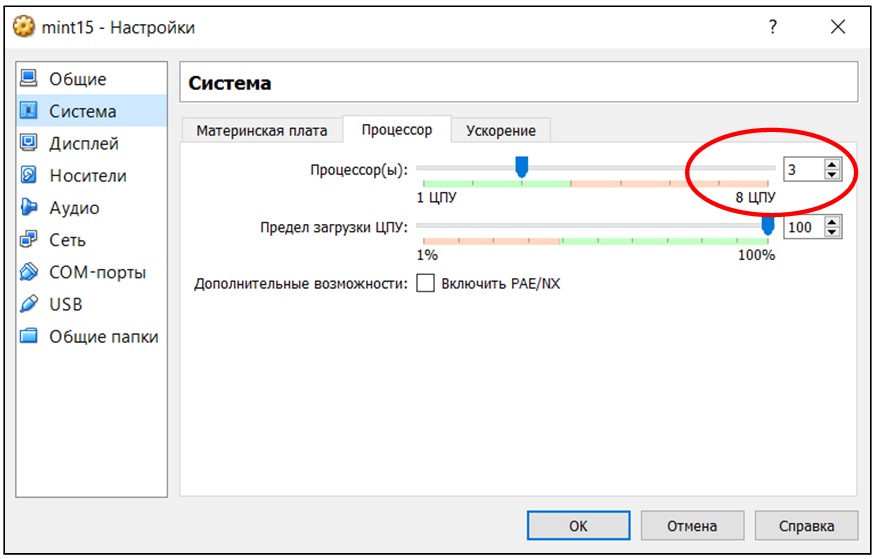
\includegraphics[width=1\linewidth]{VirtualBoxNumberCores}
		\caption{\textit{Выбор количества виртуальных процессоров в Oracle VirtualBox}}
		\label{VirtualBoxNumberCores:image}
	\end{figure}
	\parНедостатком описанного подхода являются накладные расходы виртуализации, которые непредсказуемым образом могут сказаться на результатах экспериментального измерения производительности параллельной программы. Достоинством виртуализации (по сравнению с управляемой аффинностью) является более естественное поведение тестируемой программы при использовании доступных процессоров, т.к. ОС не даётся жёстких указаний, что те или иные потоки всегда должны быть ''привязаны'' к заранее заданным процессорам (ядрам) – эта особенность позволяет более точно воспроизвести сценарий потенциального ''живого'' использования тестируемой программы, что повышает достоверность получаемых замеров производительности. 
	\par\textbf{Управление количеством нитей.} При создании параллельных программ достаточно часто количество создаваемых в процессе работы программы нитей не задаётся в виде жёстко фиксированной величины. Напротив, оно является гибко конфигурируемой величиной p, выбор значения которой позволяет оптимальным образом использовать вычислительные ресурсы той аппаратной платформы, на которой запускается программа. Это позволяет программе ''адаптироваться'' под то количество процессоров (ядер), которое есть в наличии на конкретной ЭВМ.
	\parЭту особенность параллельной программы можно использовать для экспериментального измерения её показателей эффективности, для чего параллельную программу запускают при значениях $p = 1,2,…,n$, где $n$ – это количество доступных процессоров (ядер) на используемой для тестирования многопроцессорной аппаратной платформе. Описанный подход позволяет искусственно ограничить количество используемых при работе программы процессоров (ядер), т.к. в любой момент времени параллельная программа может исполняться не более, чем на $p$ вычислителях. Анализируя измерения скорости работы программы, полученные для различных $p$, можно рассчитать значения некоторых показателей эффективности распараллеливания (см. ниже).
	\par\textbf{Параллельное ускорение (parallel speedup).} В отличие от применяемого в физике понятия величины ускорения как прироста скорости в единицу времени, в программировании под параллельным ускорением понимают безразмерную величину, отражающую прирост скорости выполнения параллельной программы на заданном количестве процессоров по сравнению с однопроцессорной системой, т.е.
	\begin{equation}
		\label{parallelAcceleration:equation}
		S(p)\;=\;\frac{V(p)}{V(1)},
	\end{equation}
	где V(p) – средняя скорость выполнения программы на $p$ процессорах (ядрах), выраженная в условных единицах работы в секунду (УЕР/с). Примерами УЕР могут быть количество просуммированных элементов матрицы, количество обработанных фильтром точек изображения, количество записанных в файл байт и т.п.
	\parСчитается, что значение $S(p)$ никогда не может превысить $p$, что на интуитивном уровне звучит правдоподобно, ведь при увеличении количества работников, например, в четыре раза невозмножно добиться выполнения работы в пять раз быстрее.  Однако, как мы рассмотрим ниже, в экспериментах вполне может наблюдаться сверх-линейное параллельное ускорение при увеличении количества процессоров. Конечно, такой результат чаще всего означает ошибку экспериментатора, однако существуют ситуации, когда этот результат можно объяснить тем, что при увеличении количества процессоров не только кратно увеличивается их вычислительный ресурс, но так же кратно увеличивается объём кэш-памяти первого уровня, что позволяет в некоторых задачах существенно повысить процент кэш-попаданий и, как следствие, сократить время решения задачи.
	\par\textbf{Параллельная эффективность (parallel efficiency).} Хотя величина параллельного ускорения является безразмерной, её анализ не всегда возможен без информации о значении $p$. Например, пусть в некотором эксперименте оказалось, что $S(p)=10$. Не зная значение $p$, мы лишь можешь сказать, что при параллельном выполнение программа стала работать в 10 раз быстрее. Однако если при этом $p=1000$, это ускорение нельзя считать хорошим достижением, т.к. в других условиях можно было добиться почти 1000 кратного прироста скорости работы и не тратить столь внушительные ресурсы на плохо распараллеливаемую задачу. Напротив, при значении $p=11$ можно было бы счесть  величину $S(p)=10$ вполне приемлемой.
	\parЭта проблема привела к необходимости определить ещё один показатель эффективности параллельной программы, который бы позволил получить некоторую оценку эффективности распараллеливания с учётом  количества процессоров (ядер). Этой величиной является \textbf{параллельная эффективность}
	\begin{equation}
		\label{parallelEffect:equation}
		E(p)\;=\;\frac{S(p)}p\;=\;\frac{V(p)}{p\cdot\;V(1)}
	\end{equation}
	\parСреднюю скорость выполнения программы $V(p)$ можно измерить следующими двумя \textit{неэквивалентными} методами:
	\begin{itemize}
		\item\textbf{Метод Амдала:} рассчитать $V(p)$, зафиксировав объём выполняемой работы (при этом изменяется время выполнения программы для различных $p$).
		\item\textbf{Метод Густавсона-Барсиса:} рассчитать $V(p)$, зафиксировав время работы тестовой программы (при этом изменяется количество выполненной работы для различных $p$).
	\end{itemize}
	Рассмотрим подробнее каждый из указанных методов в двух следующих подразделах.
	\par
}